\section{Introduction}

The Kobon triangle problem~\cite{oeis} asks for the maximum possible number of bounded triangular
faces determined by $n$ lines in the real affine plane. A classical
counting argument---each of the $n$ lines has at most $n-2$ bounded segments,
and each triangle consumes three of them---gives the upper bound
$\lfloor n(n-2)/3 \rfloor$.
For small~$n$, arrangements matching this bound can often be found by hand or
by computer search. For large~$n$, the construction of F{\"u}redi and
Pal{\'a}sti~\cite{furedi1984} asymptotically approaches the upper bound, and for
certain infinite but sparse series of~$n$ the exact maximum is known.
Constructions that produce such families are rare and especially valuable.

The general idea behind infinite series is iterative doubling: one
starts with a \emph{base configuration} of $n$ lines that is optimal and
satisfies certain geometric conditions, then inserts $n-1$ additional lines
near a distinguished line or at infinity to obtain an arrangement of $2n-1$ lines
that is again optimal and satisfies analogous conditions,
so the process can be repeated ad infinitum.

Two constructions of this type have been described in the literature,
due to Forge and Ram{\'i}rez Alfons{\'i}n \cite{forge1998} and to
Bartholdi, Blanc, and Loisel \cite{bartholdi2007}. They both yield several
affine series, including straight-line series for
\begin{equation}\label{eq:known-series}
  n = 2\cdot 2^t + 1,
  \qquad
  n = 6\cdot 2^t + 1,
  \qquad
  n = 14\cdot 2^t + 1,
  \qquad t\ge 0,
\end{equation}
and a series of affine pseudoline arrangements for
\begin{equation*}
  n = 18\cdot 2^t + 1.
\end{equation*}
A pseudoline arrangement is an arrangement of curves, not necessarily
straight, each pair crossing exactly once.
For this last family, \cite[Theorem~1.3]{bartholdi2007} gives the exact affine
upper bound
\begin{equation*}
  a_3(n)\le \left\lfloor \frac{n(n-2)}{3}\right\rfloor
  =
  \frac{n(n-2)-2}{3},
\end{equation*}
since $n\equiv 1\pmod 6$, and proves that this value is attained by affine
pseudoline arrangements.

It has remained open whether this last series can be realized by straight lines.
The main contribution of this paper is the discovery of a simple affine
arrangement of $19$ straight lines satisfying the
hypotheses of \cite[Proposition~3.1]{bartholdi2007}. This arrangement serves as
the straight-line base configuration for the iterative doubling in the case
$n=18\cdot 2^t+1$. Since the base configuration achieves the optimal triangle
count for $19$ lines, the iteration applies directly and yields the optimal
straight-line family for all $n=18\cdot 2^t+1$.

Finding the base configuration requires a systematic search. The number of
combinatorially distinct optimal arrangements grows rapidly with~$n$, while the
conditions imposed by the iterative constructions
of~\cite{forge1998,bartholdi2007} are quite restrictive: a candidate
must simultaneously be stretchable and have a specific crossing pattern
along the distinguished line or a specific pattern of slopes. We therefore organized the
computation into several stages: enumeration of optimal pseudoline arrangements,
classification up to projective equivalence, testing stretchability via
numerical optimization, and checking compatibility with the iterative constructions.

We also applied this search procedure to $n=21$, $23$, and $25$ (the last restricted to
arrangements containing a bounded pentagonal face none of whose edges belongs
to a bounded triangle). No arrangement compatible with the iterative constructions
of~\cite{forge1998,bartholdi2007} was found, providing strong computational evidence
that no further infinite straight-line families exist for
these values. For $n=21$, $23$, and $25$,
however, we found arrangements allowing a single iterative step,
yielding optimal affine arrangements for $n=41$ and $n=45$
and a projective arrangement of $49$ affine lines together with the line at infinity,
attaining the projective upper bound (Appendix~\ref{sec:appendix-one-step}).

\begin{figure}[!ht]
\centering
% Generated by Line Configuration Viewer
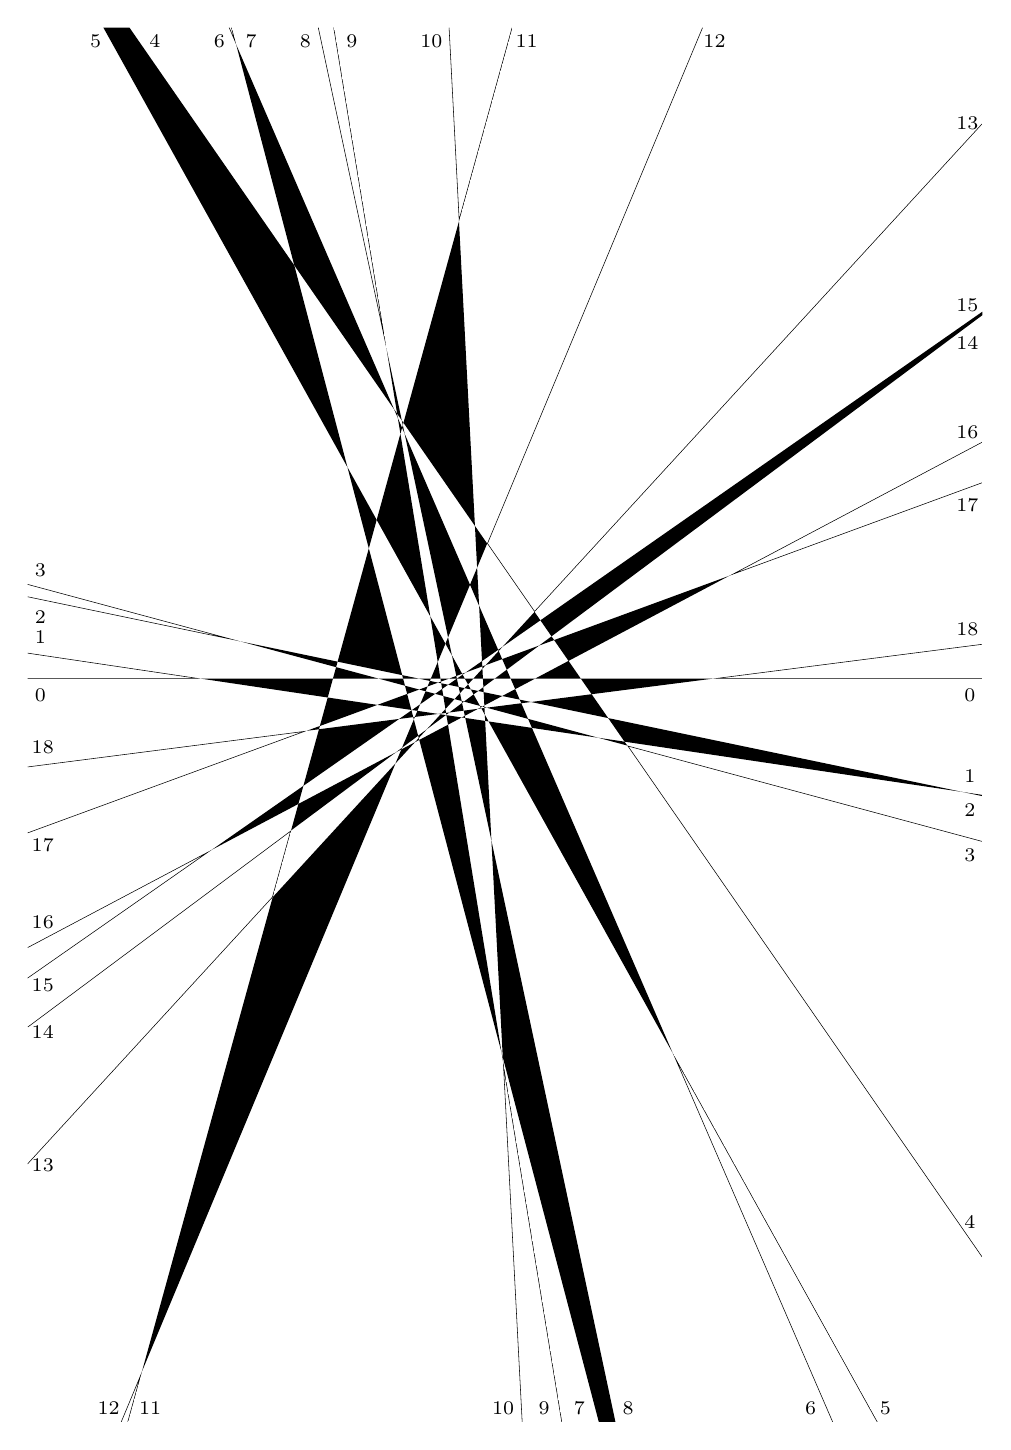
\begin{tikzpicture}[x=\linewidth,y=\linewidth]
\useasboundingbox (0,0) rectangle (1,1.46032);
\clip (0,0) rectangle (1,1.46032);
% External black cell outlines (inset)
\begin{scope}\clip (0.09767,0.00000) -- (0.10514,-0.00000) -- (0.11972,0.05287) -- cycle; \draw[line width=0.4pt] (0.10514,-0.00000) -- (0.11972,0.05287) (0.11972,0.05287) -- (0.09767,0.00000);\end{scope}
\begin{scope}\clip (0.00000,0.26992) -- (0.25660,0.54952) -- (0.27589,0.61950) -- (0.00000,0.41385) -- cycle; \draw[line width=0.4pt] (0.00000,0.26992) -- (0.25660,0.54952) (0.25660,0.54952) -- (0.27589,0.61950) (0.27589,0.61950) -- (0.00000,0.41385);\end{scope}
\begin{scope}\clip (0.00000,0.46455) -- (0.19293,0.59928) -- (0.00000,0.49713) -- cycle; \draw[line width=0.4pt] (0.00000,0.46455) -- (0.19293,0.59928) (0.19293,0.59928) -- (0.00000,0.49713);\end{scope}
\begin{scope}\clip (0.00000,0.61662) -- (0.29226,0.72385) -- (0.00000,0.68629) -- cycle; \draw[line width=0.4pt] (0.00000,0.61662) -- (0.29226,0.72385) (0.29226,0.72385) -- (0.00000,0.68629);\end{scope}
\begin{scope}\clip (0.55966,0.00000) -- (0.49782,0.37814) -- (0.51764,0.00000) -- cycle; \draw[line width=0.4pt] (0.55966,0.00000) -- (0.49782,0.37814) (0.49782,0.37814) -- (0.51764,0.00000);\end{scope}
\begin{scope}\clip (0.89010,0.00000) -- (0.67558,0.38637) -- (0.84282,0.00000) -- cycle; \draw[line width=0.4pt] (0.89010,0.00000) -- (0.67558,0.38637) (0.67558,0.38637) -- (0.84282,0.00000);\end{scope}
\begin{scope}\clip (1.00000,0.60822) -- (0.62797,0.70841) -- (1.00000,0.17182) -- cycle; \draw[line width=0.4pt] (1.00000,0.60822) -- (0.62797,0.70841) (0.62797,0.70841) -- (1.00000,0.17182);\end{scope}
\begin{scope}\clip (1.00000,0.65670) -- (0.97894,0.65984) -- (1.00000,0.65545) -- cycle; \draw[line width=0.4pt] (1.00000,0.65670) -- (0.97894,0.65984) (0.97894,0.65984) -- (1.00000,0.65545);\end{scope}
\begin{scope}\clip (-0.00000,0.77849) -- (0.18155,0.77849) -- (0.00000,0.80551) -- cycle; \draw[line width=0.4pt] (-0.00000,0.77849) -- (0.18155,0.77849) (0.18155,0.77849) -- (0.00000,0.80551);\end{scope}
\begin{scope}\clip (0.00000,0.86396) -- (0.22292,0.81748) -- (0.00000,0.87751) -- cycle; \draw[line width=0.4pt] (0.00000,0.86396) -- (0.22292,0.81748) (0.22292,0.81748) -- (0.00000,0.87751);\end{scope}
\begin{scope}\clip (0.21075,1.46032) -- (0.21833,1.44279) -- (0.21372,1.46032) -- cycle; \draw[line width=0.4pt] (0.21075,1.46032) -- (0.21833,1.44279) (0.21833,1.44279) -- (0.21372,1.46032);\end{scope}
\begin{scope}\clip (0.30409,1.46032) -- (0.37587,1.12381) -- (0.32084,1.46032) -- cycle; \draw[line width=0.4pt] (0.30409,1.46032) -- (0.37587,1.12381) (0.37587,1.12381) -- (0.32084,1.46032);\end{scope}
\begin{scope}\clip (1.00000,0.81479) -- (0.71754,0.77849) -- (1.00000,0.77849) -- cycle; \draw[line width=0.4pt] (1.00000,0.81479) -- (0.71754,0.77849) (0.71754,0.77849) -- (1.00000,0.77849);\end{scope}
\begin{scope}\clip (1.00000,1.02662) -- (0.73486,0.88623) -- (1.00000,0.98350) -- cycle; \draw[line width=0.4pt] (1.00000,1.02662) -- (0.73486,0.88623) (0.73486,0.88623) -- (1.00000,0.98350);\end{scope}
\begin{scope}\clip (1.00000,1.46032) -- (0.70655,1.46032) -- (0.48126,0.92000) -- (0.53090,0.84840) -- (1.00000,1.35954) -- cycle; \draw[line width=0.4pt] (0.70655,1.46032) -- (0.48126,0.92000) (0.48126,0.92000) -- (0.53090,0.84840) (0.53090,0.84840) -- (1.00000,1.35954);\end{scope}
\begin{scope}\clip (0.44108,1.46032) -- (0.45172,1.25742) -- (0.50764,1.46032) -- cycle; \draw[line width=0.4pt] (0.44108,1.46032) -- (0.45172,1.25742) (0.45172,1.25742) -- (0.50764,1.46032);\end{scope}
% Filled cells
\fill (0.40563,0.71191) -- (0.41013,0.71429) -- (0.40962,0.71625) -- cycle;
\fill (0.38523,0.68967) -- (0.40563,0.71191) -- (0.39135,0.70434) -- cycle;
\fill (0.39208,0.70610) -- (0.40897,0.71870) -- (0.40447,0.73581) -- cycle;
\fill (0.11972,0.05287) -- (0.38523,0.68967) -- (0.25660,0.54952) -- cycle;
\fill (0.38572,0.70136) -- (0.39135,0.70434) -- (0.39208,0.70610) -- cycle;
\fill (0.27589,0.61950) -- (0.38572,0.70136) -- (0.28354,0.64726) -- cycle;
\fill (0.38912,0.73629) -- (0.40384,0.73818) -- (0.40198,0.74527) -- cycle;
\fill (0.28877,0.66621) -- (0.38912,0.73629) -- (0.30511,0.72550) -- cycle;
\fill (0.30605,0.72890) -- (0.36629,0.75100) -- (0.31427,0.75874) -- cycle;
\fill (0.19293,0.59928) -- (0.28354,0.64726) -- (0.28877,0.66621) -- cycle;
\fill (0.29226,0.72385) -- (0.30511,0.72550) -- (0.30605,0.72890) -- cycle;
\fill (0.49648,0.38633) -- (0.49782,0.37814) -- (0.49761,0.38202) -- cycle;
\fill (0.41013,0.71429) -- (0.49648,0.38633) -- (0.44024,0.73023) -- cycle;
\fill (0.41813,0.72552) -- (0.43800,0.74033) -- (0.43248,0.74115) -- cycle;
\fill (0.40897,0.71870) -- (0.40962,0.71625) -- (0.41813,0.72552) -- cycle;
\fill (0.40555,0.73840) -- (0.42992,0.74154) -- (0.40820,0.74477) -- cycle;
\fill (0.40384,0.73818) -- (0.40447,0.73581) -- (0.40555,0.73840) -- cycle;
\fill (0.40186,0.74571) -- (0.40198,0.74527) -- (0.40248,0.74562) -- cycle;
\fill (0.43860,0.74024) -- (0.44024,0.73023) -- (0.45464,0.73786) -- cycle;
\fill (0.61561,0.00000) -- (0.48572,0.60890) -- (0.49761,0.38202) -- (0.59819,0.00000) -- cycle;
\fill (0.45833,0.73731) -- (0.48572,0.60890) -- (0.47915,0.73421) -- cycle;
\fill (0.48276,0.73367) -- (0.67558,0.38637) -- (0.52819,0.72691) -- cycle;
\fill (0.59760,0.71658) -- (0.62797,0.70841) -- (0.62514,0.71249) -- cycle;
\fill (0.36629,0.75100) -- (0.40186,0.74571) -- (0.39746,0.76244) -- cycle;
\fill (0.18155,0.77849) -- (0.31427,0.75874) -- (0.31972,0.77849) -- cycle;
\fill (0.43800,0.74033) -- (0.43860,0.74024) -- (0.43852,0.74072) -- cycle;
\fill (0.43321,0.74196) -- (0.43822,0.74260) -- (0.43755,0.74668) -- cycle;
\fill (0.42992,0.74154) -- (0.43248,0.74115) -- (0.43321,0.74196) -- cycle;
\fill (0.41105,0.75161) -- (0.42677,0.76259) -- (0.41676,0.76528) -- cycle;
\fill (0.40248,0.74562) -- (0.40820,0.74477) -- (0.41105,0.75161) -- cycle;
\fill (0.39518,0.77109) -- (0.39746,0.76244) -- (0.41009,0.76708) -- cycle;
\fill (0.45464,0.73786) -- (0.45833,0.73731) -- (0.45785,0.73955) -- cycle;
\fill (0.44163,0.74304) -- (0.45669,0.74498) -- (0.45498,0.75299) -- cycle;
\fill (0.43822,0.74260) -- (0.43852,0.74072) -- (0.44163,0.74304) -- cycle;
\fill (0.43532,0.76028) -- (0.43755,0.74668) -- (0.44712,0.75711) -- cycle;
\fill (0.47174,0.74691) -- (0.47517,0.74735) -- (0.47458,0.74841) -- cycle;
\fill (0.45669,0.74498) -- (0.45785,0.73955) -- (0.47174,0.74691) -- cycle;
\fill (0.45453,0.75511) -- (0.45498,0.75299) -- (0.45695,0.75446) -- cycle;
\fill (0.47880,0.74080) -- (0.47915,0.73421) -- (0.48276,0.73367) -- cycle;
\fill (0.47517,0.74735) -- (0.47880,0.74080) -- (0.47844,0.74777) -- cycle;
\fill (0.47373,0.74994) -- (0.47458,0.74841) -- (0.47621,0.74927) -- cycle;
\fill (0.47839,0.74869) -- (0.47844,0.74777) -- (0.48071,0.74806) -- cycle;
\fill (0.52409,0.73638) -- (0.52819,0.72691) -- (0.59760,0.71658) -- cycle;
\fill (0.36770,0.77849) -- (0.39518,0.77109) -- (0.39323,0.77849) -- cycle;
\fill (0.42677,0.76259) -- (0.43532,0.76028) -- (0.43411,0.76771) -- cycle;
\fill (0.41884,0.77029) -- (0.42986,0.77433) -- (0.42127,0.77612) -- cycle;
\fill (0.41009,0.76708) -- (0.41676,0.76528) -- (0.41884,0.77029) -- cycle;
\fill (0.44712,0.75711) -- (0.45453,0.75511) -- (0.45279,0.76328) -- cycle;
\fill (0.43314,0.77365) -- (0.43411,0.76771) -- (0.44043,0.77213) -- cycle;
\fill (0.45695,0.75446) -- (0.47373,0.74994) -- (0.46704,0.76198) -- cycle;
\fill (0.45139,0.76984) -- (0.45279,0.76328) -- (0.45761,0.76854) -- cycle;
\fill (0.47621,0.74927) -- (0.47839,0.74869) -- (0.47830,0.75038) -- cycle;
\fill (0.46416,0.76718) -- (0.46704,0.76198) -- (0.47186,0.76557) -- cycle;
\fill (0.48071,0.74806) -- (0.52409,0.73638) -- (0.51701,0.75273) -- cycle;
\fill (0.47757,0.76438) -- (0.47830,0.75038) -- (0.49706,0.76032) -- cycle;
\fill (0.51538,0.75650) -- (0.51701,0.75273) -- (0.52719,0.75403) -- cycle;
\fill (0.60802,0.73718) -- (0.62514,0.71249) -- (0.97894,0.65984) -- cycle;
\fill (0.42986,0.77433) -- (0.43314,0.77365) -- (0.43285,0.77542) -- cycle;
\fill (0.40989,0.77849) -- (0.42127,0.77612) -- (0.42226,0.77849) -- cycle;
\fill (0.44043,0.77213) -- (0.45139,0.76984) -- (0.44954,0.77849) -- cycle;
\fill (0.43235,0.77849) -- (0.43285,0.77542) -- (0.44121,0.77849) -- cycle;
\fill (0.45761,0.76854) -- (0.46416,0.76718) -- (0.46122,0.77247) -- cycle;
\fill (0.44954,0.77849) -- (0.44954,0.77849) -- (0.44955,0.77849) -- cycle;
\fill (0.47186,0.76557) -- (0.47757,0.76438) -- (0.47729,0.76962) -- cycle;
\fill (0.45788,0.77849) -- (0.46122,0.77247) -- (0.46674,0.77849) -- cycle;
\fill (0.49706,0.76032) -- (0.51538,0.75650) -- (0.51062,0.76750) -- cycle;
\fill (0.47683,0.77849) -- (0.47729,0.76962) -- (0.48920,0.77849) -- cycle;
\fill (0.52719,0.75403) -- (0.60802,0.73718) -- (0.59068,0.76219) -- cycle;
\fill (0.50586,0.77849) -- (0.51062,0.76750) -- (0.53139,0.77849) -- cycle;
\fill (0.57938,0.77849) -- (0.59068,0.76219) -- (0.71754,0.77849) -- cycle;
\fill (0.31972,0.77849) -- (0.36770,0.77849) -- (0.32303,0.79052) -- cycle;
\fill (0.22292,0.81748) -- (0.32303,0.79052) -- (0.32462,0.79628) -- cycle;
\fill (0.39226,0.78217) -- (0.39323,0.77849) -- (0.40989,0.77849) -- cycle;
\fill (0.32462,0.79628) -- (0.39226,0.78217) -- (0.35731,0.91491) -- cycle;
\fill (0.42226,0.77849) -- (0.43235,0.77849) -- (0.42951,0.79586) -- cycle;
\fill (0.33492,0.99995) -- (0.35731,0.91491) -- (0.36555,0.94479) -- cycle;
\fill (0.44121,0.77849) -- (0.44954,0.77849) -- (0.44894,0.78133) -- cycle;
\fill (0.42169,0.84368) -- (0.42951,0.79586) -- (0.43754,0.81513) -- cycle;
\fill (0.44955,0.77849) -- (0.45788,0.77849) -- (0.45555,0.78268) -- cycle;
\fill (0.44434,0.80288) -- (0.44894,0.78133) -- (0.45506,0.78357) -- cycle;
\fill (0.10665,1.46032) -- (0.07933,1.46032) -- (0.33492,0.99995) -- (0.27927,1.21134) -- cycle;
\fill (0.36555,0.94479) -- (0.42169,0.84368) -- (0.39040,1.03496) -- cycle;
\fill (0.43754,0.81513) -- (0.44434,0.80288) -- (0.44031,0.82177) -- cycle;
\fill (0.38770,1.05148) -- (0.39040,1.03496) -- (0.39214,1.04124) -- cycle;
\fill (0.46674,0.77849) -- (0.47683,0.77849) -- (0.47628,0.78889) -- cycle;
\fill (0.45878,0.78494) -- (0.47616,0.79131) -- (0.47586,0.79687) -- cycle;
\fill (0.45506,0.78357) -- (0.45555,0.78268) -- (0.45878,0.78494) -- cycle;
\fill (0.39480,1.03508) -- (0.44031,0.82177) -- (0.46328,0.87687) -- cycle;
\fill (0.48920,0.77849) -- (0.50586,0.77849) -- (0.50180,0.78789) -- cycle;
\fill (0.47970,0.79262) -- (0.49700,0.79896) -- (0.49333,0.80746) -- cycle;
\fill (0.47616,0.79131) -- (0.47628,0.78889) -- (0.47970,0.79262) -- cycle;
\fill (0.47283,0.85482) -- (0.47586,0.79687) -- (0.49279,0.80869) -- cycle;
\fill (0.38371,1.06070) -- (0.38770,1.05148) -- (0.38696,1.05602) -- cycle;
\fill (0.39214,1.04124) -- (0.39480,1.03508) -- (0.39290,1.04401) -- cycle;
\fill (0.46328,0.87687) -- (0.47283,0.85482) -- (0.47073,0.89474) -- cycle;
\fill (0.39184,1.04898) -- (0.39290,1.04401) -- (0.39358,1.04647) -- cycle;
\fill (0.53139,0.77849) -- (0.57938,0.77849) -- (0.56649,0.79708) -- cycle;
\fill (0.53571,0.81316) -- (0.55136,0.81890) -- (0.54865,0.82281) -- cycle;
\fill (0.49700,0.79896) -- (0.50180,0.78789) -- (0.53571,0.81316) -- cycle;
\fill (0.49743,0.81193) -- (0.53702,0.83958) -- (0.53090,0.84840) -- cycle;
\fill (0.49279,0.80869) -- (0.49333,0.80746) -- (0.49743,0.81193) -- cycle;
\fill (0.46844,0.93850) -- (0.47073,0.89474) -- (0.48126,0.92000) -- cycle;
\fill (0.21833,1.44279) -- (0.27927,1.21134) -- (0.38371,1.06070) -- cycle;
\fill (0.37587,1.12381) -- (0.38696,1.05602) -- (0.39184,1.04898) -- cycle;
\fill (0.39358,1.04647) -- (0.46844,0.93850) -- (0.45172,1.25742) -- cycle;
\fill (0.55136,0.81890) -- (0.56649,0.79708) -- (0.73486,0.88623) -- cycle;
\fill (1.00000,1.16290) -- (0.53702,0.83958) -- (0.54865,0.82281) -- (1.00000,1.15924) -- cycle;
% Labels
\node[inner sep=0pt,font=\scriptsize] at (0.01321,0.89186) {3};
\node[inner sep=0pt,font=\scriptsize] at (0.01321,0.84331) {2};
\node[inner sep=0pt,font=\scriptsize] at (0.01321,0.82145) {1};
\node[inner sep=0pt,font=\scriptsize] at (0.01321,0.76059) {0};
\node[inner sep=0pt,font=\scriptsize] at (0.01580,0.70623) {18};
\node[inner sep=0pt,font=\scriptsize] at (0.01580,0.60451) {17};
\node[inner sep=0pt,font=\scriptsize] at (0.01580,0.52340) {16};
\node[inner sep=0pt,font=\scriptsize] at (0.01580,0.45768) {15};
\node[inner sep=0pt,font=\scriptsize] at (0.01580,0.40772) {14};
\node[inner sep=0pt,font=\scriptsize] at (0.01580,0.26923) {13};
\node[inner sep=0pt,font=\scriptsize] at (0.98420,1.36023) {13};
\node[inner sep=0pt,font=\scriptsize] at (0.98420,1.16977) {15};
\node[inner sep=0pt,font=\scriptsize] at (0.98420,1.12956) {14};
\node[inner sep=0pt,font=\scriptsize] at (0.98420,1.03616) {16};
\node[inner sep=0pt,font=\scriptsize] at (0.98420,0.95980) {17};
\node[inner sep=0pt,font=\scriptsize] at (0.98420,0.83067) {18};
\node[inner sep=0pt,font=\scriptsize] at (0.98679,0.76059) {0};
\node[inner sep=0pt,font=\scriptsize] at (0.98679,0.67657) {1};
\node[inner sep=0pt,font=\scriptsize] at (0.98679,0.64030) {2};
\node[inner sep=0pt,font=\scriptsize] at (0.98679,0.59387) {3};
\node[inner sep=0pt,font=\scriptsize] at (0.98679,0.20877) {4};
\node[inner sep=0pt,font=\scriptsize] at (0.07113,1.44559) {5};
\node[inner sep=0pt,font=\scriptsize] at (0.13324,1.44559) {4};
\node[inner sep=0pt,font=\scriptsize] at (0.20074,1.44559) {6};
\node[inner sep=0pt,font=\scriptsize] at (0.23398,1.44559) {7};
\node[inner sep=0pt,font=\scriptsize] at (0.29085,1.44559) {8};
\node[inner sep=0pt,font=\scriptsize] at (0.33963,1.44559) {9};
\node[inner sep=0pt,font=\scriptsize] at (0.42288,1.44559) {10};
\node[inner sep=0pt,font=\scriptsize] at (0.52255,1.44559) {11};
\node[inner sep=0pt,font=\scriptsize] at (0.71938,1.44559) {12};
\node[inner sep=0pt,font=\scriptsize] at (0.08484,0.01473) {12};
\node[inner sep=0pt,font=\scriptsize] at (0.12818,0.01473) {11};
\node[inner sep=0pt,font=\scriptsize] at (0.49790,0.01473) {10};
\node[inner sep=0pt,font=\scriptsize] at (0.54087,0.01473) {9};
\node[inner sep=0pt,font=\scriptsize] at (0.57793,0.01473) {7};
\node[inner sep=0pt,font=\scriptsize] at (0.62885,0.01473) {8};
\node[inner sep=0pt,font=\scriptsize] at (0.82006,0.01473) {6};
\node[inner sep=0pt,font=\scriptsize] at (0.89830,0.01473) {5};
\end{tikzpicture}
\caption{The base configuration for $n=19$ straight lines.
}
\label{fig:base-configuration}
\end{figure}

The structure of the paper is as follows. In
Section~\ref{sec:input-statement} we recall the hypotheses of the iterative
construction from \cite{bartholdi2007}. Section~\ref{sec:combinatorics} defines
the $\mathrm{O}$-matrix encoding of the combinatorial type.
The straight-line base configuration is
established in Section~\ref{sec:main-result}, and
Section~\ref{sec:series} applies the iterative construction to derive the
infinite straight-line family. Section~\ref{sec:search} describes the computer
search that produced the base configuration, and
Section~\ref{sec:discussion} discusses the search for base
configurations at other values of~$n$.
Appendix~\ref{sec:certified-package} describes the computer-assisted
verification, and Appendix~\ref{sec:appendix-one-step} records one-step
iterative examples at $n=41$, $45$, and $49$.
